\documentclass[12pt,letter]{article}
% \usepackage[utf8]{inputenc}
\usepackage{graphicx}
\usepackage{amsmath}
\usepackage{amssymb}
\usepackage[left=2cm,right=2cm,top=3cm,bottom=2cm]{geometry}
\usepackage{float}
\usepackage[super,sort&compress,comma]{natbib} \usepackage[font={small}]{caption} %scriptsize = 8pt; footnotesize = 9pt; small = 10pt; normalsize = 11pt (set on line 4 above)
\usepackage[labelfont=bf]{caption}
\usepackage{bm}
\usepackage[T1]{fontenc}
\usepackage[version=4]{mhchem}
\usepackage{textcomp}
\usepackage{titling}
 \newcommand{\textapprox}{\raisebox{0.5ex}{\texttildelow}}
\usepackage{color}
\include{MyCommand}
\newcommand{\JPH}[1]{{\color{red}{#1}}}
\usepackage{tabularx}
\usepackage{bm}
\usepackage[left]{lineno}
\linenumbers


 \setcounter{figure}{0}
 \let\oldthefigure\thefigure
 \renewcommand{\figurename}{Supplementary Figure}

\renewcommand\refname{Supplementary References}

\begin{document}
\title{Supplementary Information: Title}
\author{Joseph Heindel$^{1,2}$, Teresa Head-Gordon$^{1,2,3}$}
\date{\vspace{-10ex}}
\maketitle
\noindent
\begin{center}
$^1$Kenneth S. Pitzer Theory Center and Department of Chemistry\\
$^2$Chemical Sciences Division, Lawrence Berkeley National Laboratory\\
$^3$Departments of Bioengineering and Chemical and Biomolecular Engineering\\
University of California, Berkeley, CA, USA


corresponding author: thg@berkeley.edu
\end{center}

\newpage

 \begin{figure} [H]
    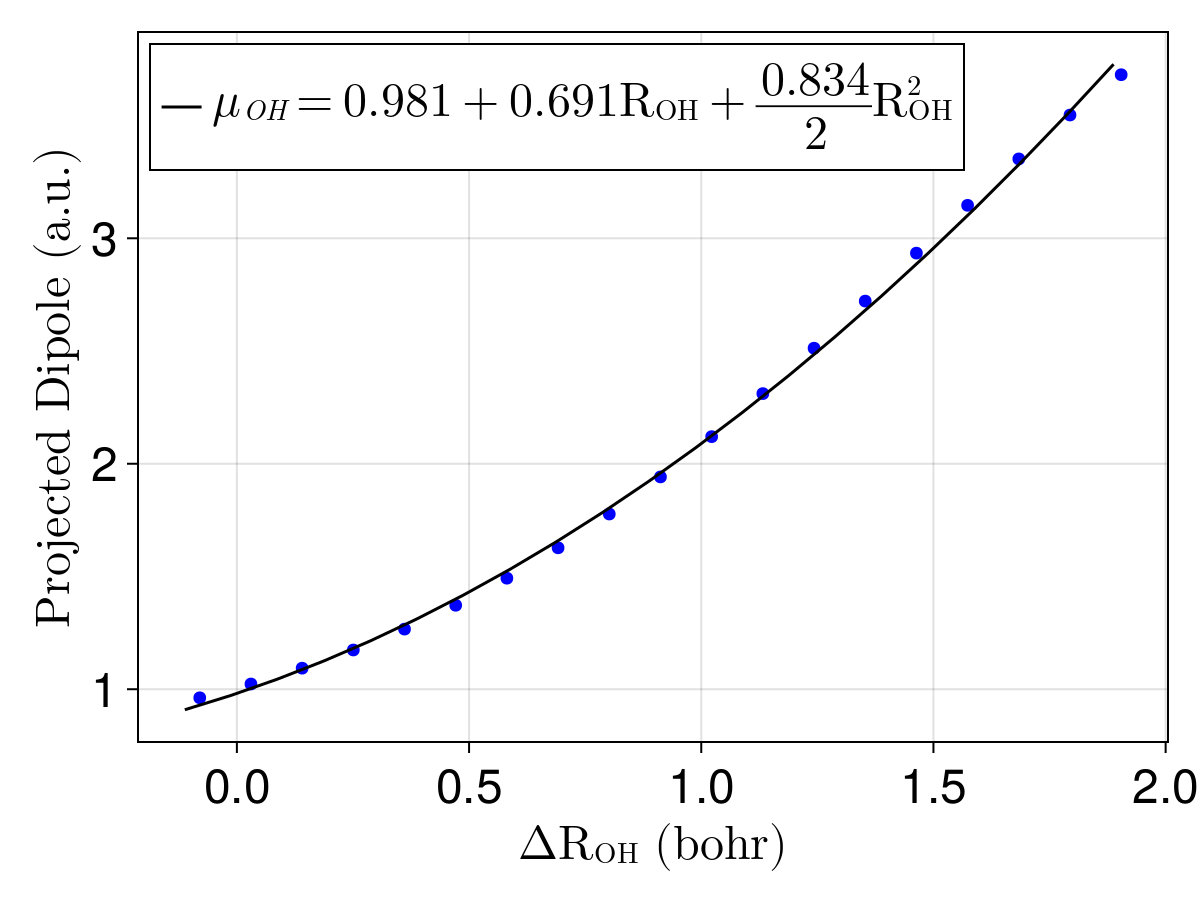
\includegraphics[width=\textwidth]{figures/dipole_derivatives_dimer.png}
    \caption{\textit{Projected dipole moment of water dimer O-H stretch}
    The dipole moment of \ce{(H2O)_2} is computed with $\omega$B97X-V/def2-QZVPPD as
    a function of the \ce{O-H} stretch distance. All other degrees of freedom are fixed.
    The dipole moment is projected along the \ce{O-H} stretch unit vector. The second
    order polynomial fit allows us to read off the corresponding dipole derivatives
    needed in the evaluation of the field-dependent morse potential.
}
    \label{fig:dip_derivatives_dimer}
\end{figure}

\bibliographystyle{unsrtnat}
\bibliography{references}
    
\end{document}
